\section{Multidimensional advection scheme}

The advection of a dependent variable $\phi$ is given by the conservation equation
\begin{align}
	\frac{\partial \phi}{\partial t} + \nabla \cdot \left( \mathbf{u} \phi \right) = 0 \label{eqn:advection}
\end{align}
where $\mathbf{u}$ is a prescribed wind field.  The time derivative is discretised using a three-stage, second-order Runge-Kutta scheme:
\begin{subequations}
\begin{align}
	\phi^\star &= \phi^{(n)} + \Delta t f(\phi^{(n)}) \\
	\phi^{\star\star} &= \phi^{(n)} + \frac{\Delta t}{2} \left( f(\phi^{(n)}) + f(\phi^\star) \right) \\
	\phi^{(n+1)} &= \phi^{(n)} + \frac{\Delta t}{2} \left( f(\phi^{(n)}) + f(\phi^{\star\star}) \right)
\end{align}
\end{subequations}
where \(f(\phi^{(n)}) = - \nabla \cdot (\mathbf{u} \phi^{(n)})\) at time level \(n\).

Using the finite volume method, the wind field is prescribed at face centroids and the dependent variable is stored at cell centroids.  The divergence term in equation~\eqref{eqn:advection} is discretised using Gauss's theorem:
\begin{align}
	\nabla \cdot \left( \mathbf{u} \phi \right) \approx \frac{1}{\mathcal{V}_c} \sum_{f \in c} \mathbf{u}_f \cdot \mathbf{S}_f \phi_F
\end{align}
where $\mathcal{V}_c$ is the cell volume, $\mathbf{u}_f$ is a wind vector prescribed at a face, ${\mathbf{S}_f}$ is the surface area vector with a direction outward normal to the face and a magnitude equal to the face area, and $\sum_{f \in c}$ denotes a summation over all faces $f$ belonging to cell $c$.  The value of the dependent variable at the face, $\phi_F$, is approximated by a least squares fit over a stencil of surrounding cell centre values.

\begin{figure}
	\centering
	\includegraphics{../fig-upwind-stencil/fig-upwind-stencil.pdf}
	\caption{An upwind-biased stencil on a two-dimensional rectangular grid.  The stencil is used to fit a multidimensional polynomial to twelve cell centred values, $\phi_c$, marked by grey circles, in order to approximate the value $\phi_F$ at the face centroid marked by an open circle.  $\phi_u$ and $\phi_d$ are the values at the centroids of the upwind and downwind cells neighbouring the target face, drawn with a heavy line.  The wind vector $\mathbf{u}_f$ is prescribed at face $f$ and determines the choice of stencil at each timestep.}
	\label{fig:interiorQuadStencil}
\end{figure}

To introduce the approximation method, we will consider how an approximate value is calculated for a face that is far away from the boundaries of a two-dimensional uniform rectangular mesh.  For any mesh, every interior face connects two adjacent cells.  The wind direction at the face determines which of the two adjacent cells is the upwind cell.  Since the stencil is upwind-biased, two stencils must be constructed for every interior face, and the appropriate stencil is chosen for each face depending on the wind direction at that face for every timestep.

The upwind-biased stencil for a face $f$ is shown in figure~\ref{fig:interiorQuadStencil}.  The wind at the face, $\mathbf{u}_f$, is blowing from the upwind cell $c_u$ to the downwind cell $c_d$.
To obtain an approximate value at $f$, a polynomial least squares fit is calculated using the stencil values.
The stencil has \num{4} points in $x$ and \num{3} points in $y$, leading to a natural choice of polynomial that is cubic in $x$ and quadratic in $y$:
\begin{align}
	\phi = a_1 + a_2 x + a_3 y + a_4 x^2 + a_5 xy + a_6 y^2 + a_7 x^3 + a_8 x^2 y + a_9 x y^2 \label{eqn:fullPoly}
\end{align}
A least squares approach is needed because the system of equations is overconstrained, with \num{12} stencil values but only \num{9} polynomial terms.  If the stencil geometry is expressed in a local coordinate system with the face centroid as the origin, then the approximated value $\phi_F$ is equal to the constant term $a_1$.

The remainder of this section generalises the the approximation technique for arbitrary meshes, explaining the methods for constructing stencils, performing a least squares fit with a suitable polynomial, and ensuring numerical stability of the advection scheme.

\subsection{Stencil construction}
For every interior face, two stencils are constructed, one for each of the possible upwind cells.  For a given face $f$ and upwind cell $c_u$, we find those faces that are connected to $c_u$ and `oppose' face $f$.  These are called the \textit{opposing faces}.
The opposing faces for face $f$ and upwind cell $c_u$ are determined as follows.
Defining $G$ to be the set of other faces bounding cell $c_u$, we calculate the `opposedness', $\mathrm{Opp}$, between faces $f$ and $g \in G$, defined as
\begin{align}
	\mathrm{Opp}(f, g) \equiv - \frac{\mathbf{S}_f \cdot \mathbf{S}_g}{|\mathbf{S}_f|^2} \label{eqn:opp}
\end{align}
where $\mathbf{S}_f$ and $\mathbf{S}_g$ are the surface area vectors pointing outward from cell $c_u$ for faces $f$ and $g$ respectively.
Using the fact that $\mathbf{a} \cdot \mathbf{b} = |\mathbf{a}|\:|\mathbf{b}| \cos(\theta)$ we can rewrite equation~\eqref{eqn:opp} as
\begin{align}
	\mathrm{Opp}(f, g) = - \frac{|\mathbf{S}_g|}{|\mathbf{S}_f|} \cos(\theta)
\end{align}
where $\theta$ is the angle between faces $f$ and $g$.  In this form, it can be seen that $\mathrm{Opp}$ is a measure of the area of $g$ and how closely it parallels face $f$.

The set of opposing faces, $\mathrm{OF}$, is a subset of $G$, comprising those faces with $\mathrm{Opp} \geq 0.5$, and the face with the maximum opposedness.  Expressed in set notation, this is
\begin{align}
	\mathrm{OF}(f,c_u) \equiv \{ g : \mathrm{Opp}(f, g) \geq 0.5 \} \cup \{ g : \max(\mathrm{Opp}(f, g)) \} 
\end{align}
On a two-dimensional rectangular mesh, there is always one opposing face that is exactly parallel to the face $f$.

Once the opposing faces have been determined, the set of internal and external cells must be found.  The \textit{internal cells} are those cells that are connected to the opposing faces.  Note that $c_u$ is always an internal cell.  The \textit{external cells} are those cells that share vertices with the internal cells.  Note that $c_d$ is always an external cell.  Having found these two sets of cells, the stencil is constructed to comprise all internal and external cells.

\begin{figure}
	\centering
	\includegraphics{../fig-double-upwind-stencil/fig-double-upwind-stencil.pdf}
	%
	\caption{A thirteen-cell, upwind-biased stencil for face $f$ connecting the pentagonal upwind cell, $c_u$, and the downwind cell $c_d$.  The dashed lines denote the two faces of cell $c_u$ that oppose $f$, and black circles mark the centroids of the internal cells that are connected to these two opposing faces.  The stencil is extended outwards by including cells that share vertices with the three internal cells, where black squares mark these vertices.  The local coordinate system $(x, y)$ has its origin at the centroid of face $f$, marked by an open circle, with $x$ normal to $f$ and $y$ perpendicular.}
	\label{fig:double-upwind-stencil}
\end{figure}

Figure~\ref{fig:double-upwind-stencil} illustrates a stencil construction for face $f$ connecting upwind cell $c_u$ and downwind cell $c_d$.  The two opposing faces are denoted by thick dashed lines and the centres of the three adjoining internal cells are marked by black circles.  The stencil is extended outwards by including the external cells that share vertices with the internal cells, marked by black squares.  The resultant stencil contains 13 cells.


\subsection{Least squares fit}
To calculate an approximate value at face $f$, a polynomial least squares fit is calculated from a stencil of surrounding cell centre values.

\TODO{what follows is not generalised: we haven't put weights on the central cells}

For faces that are far away from the boundaries of a rectangular mesh, we fit the multidimensional polynomial given by equation~\eqref{eqn:fullPoly} that has nine unknown coefficients, $\mathbf{a} = a_1 \ldots a_9$, using the twelve cell centre values from the upwind-biased stencil, $\bm{\phi} = \phi_1 \ldots \phi_{12}$.  This yields a matrix equation
\begin{align}
	\begin{bmatrix}
		1 & x_1 & y_1 & x_1^2 & x_1 y_1 & y_1^2 & x_1^3 & x_1^2 y_1 & x_1 y_1^2 \\
		1 & x_2 & y_2 & x_2^2 & x_2 y_2 & y_2^2 & x_2^3 & x_2^2 y_2 & x_2 y_2^2 \\
		\vdots & \vdots & \vdots & \vdots & \vdots & \vdots & \vdots & \vdots & \vdots \\
		1 & x_{12} & y_{12} & x_{12}^2 & x_{12} y_{12} & y_{12}^2 & x_{12}^3 & x_{12}^2 y_{12} & x_{12} y_{12}^2 \\
	\end{bmatrix}
	\begin{bmatrix}
		a_1 \\
		a_2 \\
		\vdots \\
		a_9
	\end{bmatrix}
	=
	\begin{bmatrix}
		\phi_1 \\
		\phi_2 \\
		\vdots \\
		\phi_{12}
	\end{bmatrix}
\end{align}
which can be written as $\mathbf{B} \mathbf{a} = \bm{\phi}$.
The rectangular matrix $\mathbf{B}$ has one row for each cell in the stencil and one column for each term in the polynomial, and $\mathbf{B}$ is constructed using only the mesh geometry.
A local coordinate system is established in which $x$ is normal to the face $f$ and $y$ is perpendicular to $x$.
The coordinates $(x_i, y_i)$ give the position of the centroid of the $i$th cell in the stencil.
The unknown coefficients $\mathbf{a}$ are calculated using the pseudo-inverse of $\mathbf{B}^+$ found by singular value decomposition:
\begin{align}
	\mathbf{a} = \mathbf{B}^+ \bm{\phi}
%
\intertext{Recall that the approximate value $\phi_F$ is equal to the constant coefficient $a_1$, which is calculated as} 
%
	a_1 = \begin{bmatrix}
		b_{1,1}^+ \\
		b_{1,2}^+ \\
		\vdots \\
		b_{1,12}^+
	\end{bmatrix}
	\cdot
	\begin{bmatrix}
		\phi_1 \\
		\phi_2 \\
		\vdots \\
		\phi_{12}
	\end{bmatrix}
\end{align}
where $b_{1,1}^+ \ldots b_{1,12}^+$ are the elements in the first row of $\mathbf{B}^+$.

For faces of a non-rectangular mesh, or faces that are near a boundary, the number of stencil cells and number of polynomial terms may differ: a stencil will have two or more cells and, for two-dimensional meshes, its polynomial will have between one and nine terms.  Additionally, the polynomial cannot have more terms than its stencil has cells because this would lead to an underconstrained system of equations.  The procedure for choosing suitable polynomials is discussed next.

\subsection{Polynomial generation}
% generating candidates
% full rank check

\subsection{Stabilisation procedure}
% stability constraints
% reweighting

Stability constriants:
\begin{align}
	0.5 \leq u \leq 1 \\
	0 \leq d \leq 0.5 \\
	u - d \geq \max(|p|)
\end{align}

\begin{figure}
	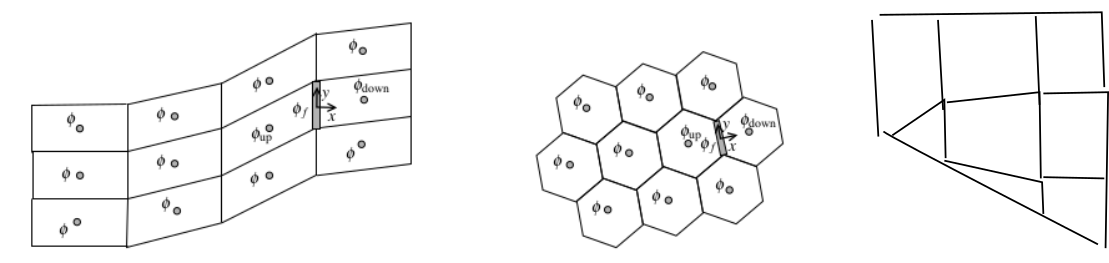
\includegraphics[width=\textwidth]{stencilConstruction.png}
	\caption{\TODO{example stencils in interior of quad and hex meshes, and example stencil near boundary of a slanted cell mesh (taken from one of the test cases)}}
\end{figure}
\end{document}
